\documentclass[a4paper,12pt]{article}


\providecommand{\keywords}[1]{\textbf{\textit{Keywords---}} #1}
\usepackage[pdftex]{graphicx}
\usepackage{url}
\setlength{\oddsidemargin}{0.25in}
\setlength{\textwidth}{6.5in}
\setlength{\topmargin}{0in}
\setlength{\textheight}{8.5in}
\usepackage[utf8]{inputenc}
\usepackage[english]{babel}
\usepackage{gensymb}
\usepackage[backend=biber,style=numeric,sorting=none]{biblatex}
\addbibresource{references.bib}
\usepackage{graphicx}
\usepackage{subcaption}
\usepackage{fixltx2e}
\usepackage{textgreek}
\usepackage{mathtools}
\usepackage{lscape}
\usepackage[most]{tcolorbox}
\usepackage{lipsum}


\begin{document}
\title{Design and control of a finger exoskeleton for rehabilitation with compliant actuation}
\author{Batuhan Toker}
\date{\today}
\maketitle
\begin{abstract}
\emph{This paper is a progress report for design and control of \textsc{AsistOn-Finger} with  \textsc{HandsOn} actuation modules. Human rehabilitation is often better handled by control of force of interaction between assisted extremity and the environment instead of simply controlling the position of the end-effector. Compliant actuation is used in such designs to minimize large forces due to shocks, obtain safe interaction with user and environment, store and release energy. Series damping elastic actuator was proposed as  \textsc{HandsOn-SDEA} to provide faster shock absorption by adding damping unit to \textsc{HandsOn-SEA}. Series damping actuator was proposed as \textsc{HandsOn-SDA} which senses exerted force by measuring damping. Passivity constraints of basic impedance control of \textsc{HandsOn-SEA} \textsc{HandsOn-SDA} and \textsc{HandsOn-SDEA} is derived. Basic impedance controller allows the system to passively render Voigt model desired impedance dynamics that is not allowed to be passively rendered in velocity sourced impedance control. In physical human-robot interaction, it is a necessary to passively render any passive impedance, which will be guaranteed by basic impedance control.}
\end{abstract}
\keywords{series elastic actuator,series damping actuator, series damping elastic actuator, force control,impedance control}

\section{Introduction}

All living organisms have the ability of interacting with the environment. Human body has a pair of highly skilled mechanism that allows us to interact with and modulate the environment, as known as hand. Human hand has capability to perform complex movements with a complicated structure consisting of 27 bones and bunch of muscles. The human hand provides tactile feedback by nerves. This force feedback is used by the brain and used to determine the mechanical properties of objects while manipulating the objects\cite{BIANCHI20188}. 

There are many people all over the world who receive physical treatments for hand and finger injuries. The most common region injured is the finger\cite{daan}. These injuries are difficult to impair due to the complexity of human fingers. After an injury, the fingers may loose its functionality due to non-proper treatment. The hand can regain its functionality after an injury by an occupational or physical therapy. Robotic devices are used to reduce cost of therapies, meanwhile providing more accuracy in the therapeutic exercises. The most basic type of therapy devices are non-actuated devices such as Thera-Band \cite{thera}, Digiflex \cite{digiflex}. These devices provide help in grasping of the hand or extension/flexion motion of the fingers. Continous passive motion (CPM) devices are another type for hand therapies, which constantly move the joint through desired range of motion\cite{SCHWARTZ2006448}.

In addition to these devices, there are various finger/hand exoskeleton devices have been developed for physical therapy of upper extremity\cite{kawasakihapt}\cite{lucas}\cite{frisoli}. The main purpose of cumulative development in upper limb exoskeleton field is to achieve a design like skillful human hand. For the last decades, the field of upper limb exoskeleton has become a challenging topic for design engineering. Recent developments in actuation mechanisms and material sciences are promising some advantages for patients and physical therapists by providing them bio-mimetic exoskeletons. These developments have provided considerable progress in terms of their degree of freedom (DoF), weight, size, and skillful manipulation\cite{Heo2012}.

Exoskeletons are such devices that directly interact with the human body. The literature shows that force control based devices are more effective in rehabilitation devices for both the upper\cite{Blank2014} and lower limbs\cite{Marchal-Crespo2009}, instead of position based control devices\cite{harwin}. Force based control in therapy devices can be designed to ensure active effort from the patient during the therapy, which is more effective than passive motor training\cite{lotze}. However, position based control in therapy devices strictly follow a desired trajectory without enabling the patient to actively involve in the task by guiding the movement of the impaired limb\cite{Bernhardt2005HybridFC}\cite{agarwalindex}. Force feedback is important because the patient should understand the surroundings and manipulates objects according to the transmitted force information\cite{jobae}. To provide this force feedback, a force sensor may be used in the exoskeleton, but recent force sensors are so large and heavy. A lightweight and safe actuation mechanism is necessary for the finger exoskeleton system. Due to requirements of the device, series elastic actuation (SEA) mechanism with an electric motor is used as actuation module to satisfy both safety and weight requirements. Such mechanism provides measuring the transmitted force by the spring deflection between the actuator and the human side. Defined mechanical stiffness is combined with proper sensors to measure force exerted by the external environment to the mechatronic system. SEA stores an energy load during the interaction, and provides the safety in human machine interaction\cite{BIANCHI20188}. Series elastic actuator ensures a good torque or force control with low mass for exoskeletons. There have been many attempts to develop series elastic actuated hand exoskeleton systems \cite{jobae}\cite{inseongbae}\cite{BIANCHI20188}\cite{agarwalindex} .

In this project, a wearable and force controllable finger exoskeleton is proposed to meet low inertia and safety requirements in tendon therapy. The device will be built on \textsc{AsistOn-Finger}\cite{ertas}  and will be driven by \textsc{HandsOn-SEA}\cite{handsonsea}. For hand rehabilitation, bidirectional peak torque is defined as at least 0.3 Nm based on the torques applied by professional therapists \cite{Ueki2012DevelopmentOA}. Bandwidth will be limited to at least 2 Hz, according to the fact that human force compliance control loop bandwidth is 1-2 Hz\cite{chan}\cite{sheridan}. Typical rehabilitation therapies for the finger are implemented at angular velocities of 50\degree/s, for example full range of motion frequencies below 0.5 Hz\cite{Adamovich}\cite{kawasaki}. 
Passivity analysis of BIC is completed for three different compliant actuator.  
\section{Design}
\subsection{\textsc{HandsOn-SEA}}\\

\textsc{AsistOn-Finger} is a novel, under-actuated active exoskeleton for robot assisted tendon therapy for human fingers. The main purpose in the design of this device is to assist flexion and extension motions of a finger within its range of motion. The tendon therapy device will be driven by \textsc{HandsOn-SEA}. The handle of \textsc{HandsOn-SEA} will be the actuated linkage of the \textsc{AsistOn-Finger}. The linear analog model for the system is represented in the Figure~\ref{fig:model}.
\begin{figure}[h]
\centering
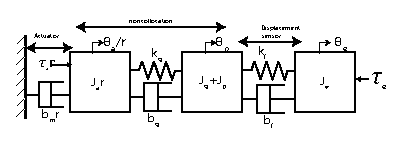
\includegraphics[scale=2]{sea.eps}
\caption{A linear analog of the system model of SEA connected to the tendon device. In this model J\textsubscript{a} is the inertia of the motor, J\textsubscript{g} is the inertia of power transmission module, J\textsubscript{p} is the inertia of the sector pulley about the bearing, J\textsubscript{e} is the total inertia of the tendon device, r is the reduction ratio of the power transmission, k\textsubscript{g} and b\textsubscript{g} signify the inertia distribution between J\textsubscript{a} and J\textsubscript{g}, k\textsubscript{f} and b\textsubscript{f} signify the force sensor -in this case this is a displacement sensor with a spring- attached to actuated linkage that interacts with the environment, \texttau  \textsubscript{a} is the torque exerted by the motor and \texttau  \textsubscript{e} is the torque exerted by the environment }
\label{fig:model}
\end{figure}

DC motor's motion is controlled by regulating its voltage. The torque constant of the DC motor is defined as K\textsubscript{m}, R is  the motor resistance,  K\textsubscript{b} is the motor back-emf constant, and b\textsubscript{m} is the cumulative damping of the motor. The transfer function from motor voltage V(s) to motor velocity s\texttheta\textsubscript{m}(s) can be derived as following:
\begin{equation}
\frac{s\theta_m(s)}{V(s)}=\frac{\frac{K_m}{R}}{Js+b}
\end{equation}
where \(J=J_a+J_g+J_p/r^2\) and \(b=b_m+\frac{K_mK_b}{R}\).

J\textsubscript{e} is neglected, because its inertia is orders of magnitude smaller than the reflected intertia of the motor side of the cross-flexure pivot. After neglecting J\textsubscript{e}, the torque \texttau  \textsubscript{e} measured by the flexure acts on the system by following equation
\begin{equation}
\frac{s\theta_m(s)}{\tau_e(s)}=\frac{\frac{-1}{R}}{Js+b}
\end{equation}
where rotation of the pulley is \(\theta_p(s)=\frac{\theta_m(s)}{r}\)
\begin{table}[h]
\centering
\begin{tabular}{@{}lll@{}}
\hline
\multicolumn{3}{c}{Parameters of \textsc{HandsOn-SEA}} \\ 
\multicolumn{1}{l|}{J_a - \text{inertia of the motor}} & \multicolumn{1}{l|}{1.3} & gr-cm^2 \\ 
\multicolumn{1}{l|}{J_g - \text{inertia of the gearhead}} & \multicolumn{1}{l|}{0.05} & gr-cm^2 \\
\multicolumn{1}{l|}{J_h - \text{inertia of the of handle about the bearing}} & \multicolumn{1}{l|}{1.93} & gr-cm^2 \\
\multicolumn{1}{l|}{J_p - \text{inertia of the sector pulley about the bearing}} & \multicolumn{1}{l|}{14.7} & gr-cm^2 \\
\multicolumn{1}{l|}{r_g - \text{gearhead reduction ratio}} & \multicolumn{1}{l|}{84:1} &  \\
\multicolumn{1}{l|}{r_c - \text{capstan reduction ratio}} & \multicolumn{1}{l|}{73:9} &  \\
\multicolumn{1}{l|}{k_f - \text{stiffness of sensor}} & \multicolumn{1}{l|}{5000} & N-mm/rad  \\
\multicolumn{1}{l|}{L - \text{motor inductance}} & \multicolumn{1}{l|}{0.452} &  mH \\
\multicolumn{1}{l|}{R- \text{motor resistance}} & \multicolumn{1}{l|}{10.7} & Ohm \\
\multicolumn{1}{l|}{b_m - \text{cumulative damping of the motor}} & \multicolumn{1}{l|}{0.0025} & N-mm/s \\
\multicolumn{1}{l|}{K_m - \text{motor torque constant}} & \multicolumn{1}{l|}{16.2} & mN-m/A \\
\multicolumn{1}{l|}{K_b - \text{motor back-emf constant}} & \multicolumn{1}{l|}{61.7} & rad/sec/A \\
\multicolumn{1}{l|}{$\tau$_m - \text{mechanical time constant}} & \multicolumn{1}{l|}{5.31} & ms \\
                      &                       & 
\end{tabular}
\end{table}
\subsection{\textsc{HandsOn-SDEA/SDA}}
The \texttau  \textsubscript{e} is represented as work piece dynamics
\begin{equation}
\tau_{e}(s)=m_ws^2+b_ws+k_w
\end{equation}
\begin{figure}[h]
\centering
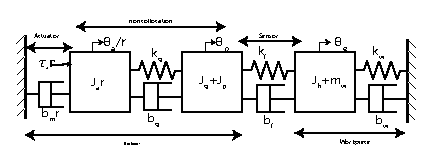
\includegraphics[scale=2]{seav2.eps}
\caption{A linear analog of the system model of a compliant actuator connected to the tendon device. In this model \texttau  \textsubscript{e} is represented as work piece dynamics}
\label{fig:model2}
\end{figure}
This analog model has the following open loop transfer functions\cite{eppinger}:
\begin{equation}
\frac{\theta_a(s)/r}{\tau_a(s)r}=\frac{4^{th}\text{order numerator polynomial}}{6^{th}\text{order numerator polynomial}}
\end{equation}
\begin{equation}
\frac{\theta_p(s)}{\tau_a(s)r}=\frac{3^{rd}\text{order numerator polynomial}}{6^{th}\text{order numerator polynomial}}
\end{equation}
\begin{equation}
\frac{\theta_e(s)}{\tau_a(s)r}=\frac{2^{nd}\text{order numerator polynomial}}{6^{th}\text{order numerator polynomial}}
\end{equation}
where 
\begin{equation}
\begin{multlined}\\
\text{the second order polynomial } = [b_gs+k_g][b_fs+k_f]\\
\text{the third order polynomial } = [b_gs+k_g][\tau_{e}(s)+J_hs^2]\\
\text{the fourth order polynomial } = [(J_g+J_p)s^2+(b_g+b_f)s+(k_g+k_f)][\tau_{e}(s)+J_hs^2]-[b_gs+k_g]^2 \\
\text{the sixth order polynomial } = [J_as^2+(b_m+b_g)s+k_g][(J_g+J_p)s^2+(b_g+b_f)s+(k_g+k_f][\tau_{e}(s)\\+J_hs^2]-[\tau_{e}(s)+J_hs^2][b_gs+k_g]^2-[J_as^2+(b_m+b_g)s+k_g][b_gs+k_g]^2
\end{multlined}
\end{equation}
\begin{figure}[h]
\centering
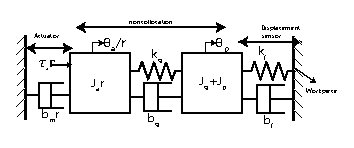
\includegraphics[scale=2]{seav3.eps}
\caption{A linear analog of the system model of a compliant actuator connected to the tendon device. In this model \texttau  \textsubscript{e} is modeled rigidly as a "wall".}
\label{fig:model3}
\end{figure}
Figure~\ref{fig:model3} represents the compliant actuator. In this model, the workpiece dynamics are excluded. The open loop transfer function for this model is:
\begin{equation}
\frac{\theta_p(s)}{\tau_a(s)r}=\frac{1^{st}\text{order numerator polynomial}}{New 4^{th}\text{order numerator polynomial}}
\end{equation}
where 
\begin{equation}
\begin{multlined}\\
\text{the new fourth order polynomial } = [J_as^2+(b_m+b_g)s+k_g][(m_2)s^2+(b_g+b_f)s+(k_g+k_f]\\-[b_gs+k_g]^2\\
\text{the new first order polynomial } = [b_gs+k_g]\\
\end{multlined}
\end{equation}
where $m_2=J_g+J_p/(r_g*r_p)^2$ and $k_g=k_f/r_g$\\
For further simplification, non collocation in the actuator allows us to model the actuator with transfer function of
\begin{equation}
G_{actuator}=\frac{\theta(s)}{\tau_a(s)}=\frac{1}{J_ms^2+b_ms}
\end{equation}
For the dynamic models of different type of actuators the torque estimation by the torque sensor will be defined as:\\
For series elastic actuator,
\begin{equation}
\tau_{sens}(s)=k_f(\theta_p-\theta_h)
\end{equation}
for series damping elastic actuator,
\begin{equation}
\tau_{sens}(s)=k_f(\theta_p-\theta_h)+b_f(\dot\theta_p-\dot\theta_h)s
\end{equation}
and for series damping actuator
\begin{equation}
\tau_{sens}(s)=b_f(\dot\theta_p-\dot\theta_h)s
\end{equation}

The kinematic analysis of the tendon device will be explained in this section in part of future work. The optimal dimensions synthesized in\cite{ertas} will be used to have a dynamic model for the tendon device.

\section{Force Control of compliant actuators}
\subsection{Velocity Sourced Impedance Controller}\\
\textsc{HandsOn-SEA} is controlled by the cascaded controller architecture which is based on Velocity-Sourced Impedance Control\cite{tagliamonte} is represented in Figure~\ref{fig:handson}. This controller architecture is consist of an inner velocity control loop and an intermediate force control loop and an outer impedance control loop. The imperfections of the power transmission system is compensated by inner loop. Modelling errors such as friction, stiction and slip are eliminated by robust motion controller. Force tracking performance is ensured by intermediate control loop by using force feedback. The outer loop determines the effective output impendance of the system. The controller parameters are defined to satisfy passivity of interaction\cite{tagliamonte}.


\begin{figure}[h]
\centering
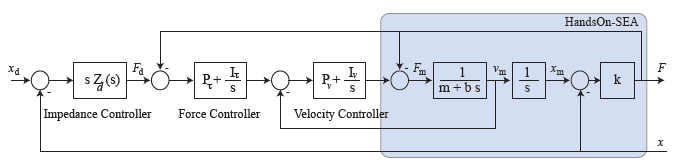
\includegraphics[scale=0.6]{Untitled.png}
\caption{Cascaded control architecture of \textsc{HandsOn-SEA}  }
\label{fig:handson}
\end{figure}
Impedance control is used in the cascaded control architecture to model dynamic relation between the actuator position and applied external force. Passivity in impedance control depends on control architecture, system dynamics and the desired impedance. For given control architecture, the set of passively rendered impedance values is called Z-width\cite{adamsblake}. The virtual inertia of the controlled motor cannot be less than the half of motor's physical inertia. This phenomena is proven by using non-collocated proportional force feedback\cite{colgate}. Also virtual stiffness of the series elastic actuator cannot be higher than physical spring stiffness, in velocity sourced impedance control (VSIC) architectures\cite{vallery}.\\

To conclude the velocity sourced impedance control\cite{calanca}
\begin{itemize}
\item There is no upper limit exist for the velocity and force proportional gains for given sufficiently low ratio of these gains.
\item Pure integrators can be used in velocity and force loops with limited integral gains. There is a trade-off between integral gain and k\textsubscript{d}.
\item For desired pure spring impedance dynamics(\(sI(s)=k_d\)), the maximum desired stiffness should be less than the physical spring to ensure passivity.
\item For desired parallel spring and damping impedance dynamics(\(sI(s)=k_d+sd_d\)), the control architecture does not ensure the passivity\cite{tagliamonte}.
\end{itemize}\\
Velocity Sourced Impedance Controller is represented in Figure~\ref{fig:model7}
\begin{figure}[h]
\centering
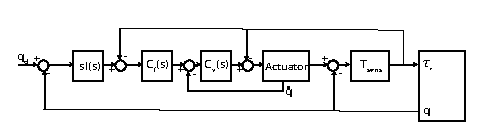
\includegraphics[scale=2]{vsic.eps}
\caption{Velocity Sourced Impedance Controller(VSIC) for sensing of \textsc{HandsOn-SEA}}
\label{fig:model7}
\end{figure}
For the VSIC case, two proportional-integral force and velocity control laws are considered:
\begin{equation}
C_{f}(s)=P_{f}+\frac{I_{f}}{s} \\
\end{equation}
\begin{equation}
C_{v}(s)=P_{v}+\frac{I_{v}}{s}  \\
\end{equation}
Torque estimation of SEA is:
\begin{equation}
\tau_{sens}(s)=k_f(\theta_p-\theta_h)
\end{equation}
so that the impedance at the environment is calculated as following
\begin{equation}
\begin{multlined}\\
\tau_e(s)=((((Z_{d}err-\tau_e(s))C_{f}-\dot{q})C_{v}-\tau_e(s))G_{actuator}-q)\tau_{sens}(s) \\
\tau_e(s)=((C_{f}Z_{d}err-C_{f}\tau_e(s)-\dot{q})C_{v}-\tau_e(s))G_{actuator}-q)\tau_{sens}(s) \\
\tau_e(s)=((C_{v}C_{f}Z_{d}err-C_{v}C_{f}\tau_e(s)-\dot{q}C_{v}-\tau_e(s))G_{actuator}-q)\tau_{sens}(s) \\
\tau_e(s)=((G_{actuator}C_{v}C_{f}Z_{d}err-\tau_e(s)(C_{v}C_{f}+1)G_{actuator}-\dot{q}C_{v}G_{actuator}-q)\tau_{sens}(s) \\
\end{multlined}\\
\end{equation}
Simplification is carried out for
\begin{equation}
\begin{multlined}\\
\dot{q}=qs\\
q_{d}=0 \\
\end{multlined}\\
\end{equation}
And the environment impedance is defined for
\begin{equation}
\tau_e(s)=-Z_{e}\dot{q}\\
\end{equation}
\begin{equation}
Z_{e}=\frac{\tau_e(s)}{-\dot{q}}=\frac{\frac{1}{s}\tau_{sens}(s)(G_{actuator}C_{v}C_{f}Z_{d}+sC_{v}G_{actuator}+1)}{1+(C_{v}C_{f}+1)G_{actuator}\tau_{sens}(s)}
\end{equation}
\subsection{Basic Impedance Controller}
In this project, I propose to implement basic impedance control to \textsc{HandsOn-SDEA}, \textsc{HandsOn-SEA} and \textsc{HandsOn-SDA}, to avoid environment uncertainties, meanwhile the violation of the integrator on the passivity of the inner force loop will be eliminated\cite{pratt}. 
The proposed controller architecture is given in Figure~\ref{fig:bic}.A paralel spring-damper dynamics were considered:
\begin{equation}
sI(s)=Z_d=k_d+sd_d  
\end{equation}
A proportional-derivative force control law is considered:
\begin{equation}
C_f(s)=P+sD  
\end{equation}
\begin{figure}[h]
\centering
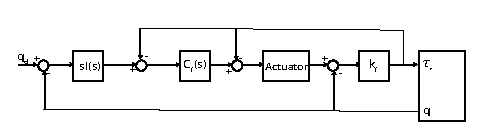
\includegraphics[scale=2]{bic.eps}
\caption{Basic Impedance Controller(BIC) for sensing of \textsc{HandsOn-SEA}}
\label{fig:bic}
\end{figure}
Block diagram for the robot block in the controller is given in Figure~\ref{fig:robot}.
\begin{figure}[h]
\centering
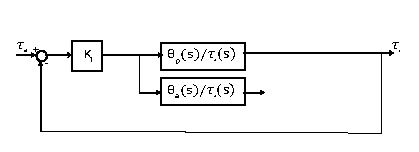
\includegraphics[scale=2]{robotv2.eps}
\caption{Block diagram of actuator}
\label{fig:robot}
\end{figure}
The impedance at the environment port (\texttau  \textsubscript{e},$\dot{q}$) will be calculated for error dynamics of
\begin{equation}
err=q_d-q
\end{equation}
Closed loop dynamics of the system will be
\begin{equation}
(((sI(s)err-\tau_{e}(s))C_f(s)-\tau_{e}(s))\frac{\theta(s)}{\tau_a(s)})-q)k_f=\tau_{e}(s)
\end{equation}
The open loop transfer function of the actuator:
\begin{equation}
G_{actuator}=\frac{\theta(s)}{\tau_a(s)}
\end{equation}
Simplifyng is carried out for $q_d=0$:
\begin{equation}
-q(k_fC_fsI(s)G_{actuator}+k_f)=\tau_{e}(s)(1+k_fG_{actuator}+C_fK_f)
\end{equation}
so that the impedance at the environment
\begin{equation}
\frac{\tau_e(s)}{-\Dot{q}(s)}=\frac{(k_fC_fI(s)G_{actuator})+k_f}{1+k_fG_{actuator}+C_fK_f}    
\end{equation}

Then the contoroller is upgraded for defined $\tau_{sens}$ in Figure~\ref{fig:model4}
\begin{figure}[h]
\centering
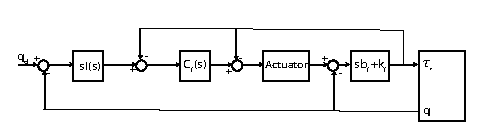
\includegraphics[scale=2]{bicv2.eps}
\caption{Basic Impedance Controller(BIC) for sensing of \textsc{HandsOn-SDEA}}
\label{fig:model4}
\end{figure}
the impedance at the environment for this controller will be
\begin{equation}
\frac{\tau_e(s)}{-\Dot{q}(s)}=\frac{(b_fs+k_f)C_fI(s)G_{actuator}+b_fs+k_f}{1+(b_fs+k_f)(G_{actuator}+C_f)}   
\end{equation}
\begin{figure}[h]
\centering
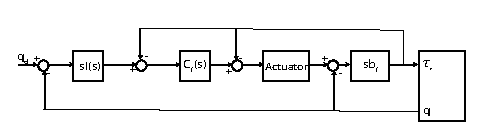
\includegraphics[scale=2]{bicv3.eps}
\caption{Basic Impedance Controller(BIC) for sensing of \textsc{HandsOn-SDA}}
\label{fig:model5}
\end{figure}
Finally, basic impedance controller for \textsc{HandsOn-SDA} is represented in Figure~\ref{fig:model5}. The impedance at the environment in the control of the actuator will be 
\begin{equation}
\frac{\tau_e(s)}{-\Dot{q}(s)}=\frac{(b_fs)C_fI(s)G_{actuator}+b_fs}{1+(b_fs)(G_{actuator}+C_f)}   
\end{equation}
The environment impedance of BIC can be generalized as following
\begin{equation}
\frac{\tau_e(s)}{-\Dot{q}(s)}=\frac{\frac{\tau_{sens}}{s}(C_fZ_{d}G_{actuator}+1)}{1+G_{actuator}\tau_{sens}(C_f+1)}   
\end{equation}
\newpage
\section{Passivity analysis}

The passivity conditions will be derived for basic impedance control and velocity sourced impendace control of \textsc{HandsOn-SEA/SDEA/SDA} will be presented in this section.\\

\subsection{Passivity analysis of VSIC}
\subsubsection{Passivity analysis of VSIC for \textsc{HandsOn-SEA}}
\begin{equation}
\tau_{sens}(s)=k_f(\theta_p-\theta_h)
\end{equation}

Desired stiffness $k_d$ cannot be smaller than the sensor stiffness $k_f$\cite{calanca} for desired impedance of pure spring. Additionally;
\begin{equation}
I_f+I_v(\frac{P_f}{P_v})\leq \frac{P_fP_v}{J_m}
\end{equation}\\

This controller cannot ensure passivity for VM impedance\cite{tagliamonte}.
\subsection{Passivity analysis of BIC}
\subsubsection{Passivity analysis for BIC for \textsc{HandsOn-SEA}}
\begin{equation}
\tau_{sens}(s)=k_f(\theta_p-\theta_h)
\end{equation}
\begin{equation}
\frac{\tau_e(s)}{-\Dot{q}(s)}=\frac{(k_fC_fI(s)G_{actuator})+k_f}{1+k_fG_{actuator}+C_fK_f}    
\end{equation}
For defined function of force sensing the environmet impedance will be 
\begin{equation}
\begin{multlined}\\
Z_{e}(s)=\frac{\tau_e(s)}{-\Dot{q}(s)}=\frac{\frac{k_{f}}{s}(C_fZ_{d}G_{actuator}+1)}{1+G_{actuator}k_{f}(C_f+1)} \\
Z_{e}(s)=\frac{\frac{k_{f}}{s}(C_fZ_{d}G_{actuator}+1)}{1+G_{actuator}k_{f}(C_f+1)} \\
Z_{e}(s)=\frac{\frac{k_{f}}{s}((k_d+sd_d)(P+sD)\frac{1}{J_ms^2+b_ms})+1)}{J_ms^2+b_ms+k_f(P+sD+1)}\\
Z_{e}(s)=\frac{\frac{k_{f}}{s}((k_d+sd_d)(\frac{P}{s}+D))+k_f(J_ms+b_m)}{J_ms^2+b_ms+k_f(P+sD+1)}\\
\end{multlined}\\
\end{equation}
using backward difference differentiation of position:
\begin{equation}
\begin{multlined}\\
Z_{e}(s,z)=\frac{\frac{k_{f}}{s}((k_d+d_d(\frac{z-1}{Tz}))(\frac{P}{s}+D))+k_f(J_ms+b_m)}{J_ms^2+b_ms+k_f(P+sD)}\\
Z_{e}(jw)=\frac{\frac{k_{f}}{s}((k_d+\frac{d_d}{T}+\frac{d_dj}{Tw}))(\frac{P}{jw}+D))-k_fJ_mw^2+b_mk_fj)}{-J_mw^2+b_mjw+k_f(P+jwD+1)}\\
\end{multlined}\\
\end{equation}
The complex conjugate of the den is defined as $den_{conj}=-J_mw^2-(b_m+k_fD)jw+k_f(P+1)$, the environment impedance will be in form of$Re(Z_{e})=\frac{1^{st} \mathrm{numerator}}{1^{st}\mathrm{den}}$ where\\
\begin{equation}
\begin{multlined}\\
1^{st} \mathrm{numerator}=-J_m^2w^3+(DJ_mk_f)(k_d+\frac{d_d}{T})w^2+(J_mb_m-J_mk_f(1+P))w+k_dk_f(Dk_f-Pb_m)\\+\frac{Dd_dk_f^2+D^2d_dk_f+J_mPd_dk_f+Db_md_dk_f-Pb_md_dk_f}{T}+\frac{b_mk_f+Pb_mk_f}{w}+\frac{Pd_dk_f^2+P^2d_dk_f^2}{Tw^2}\\
1^{st} \mathrm{den}=J_m^2w^4+(D^2k_f^2+2Db_mk_f+2J_mPk_f+2J_mk_f+b_m^2)w^2+k_f^2(P^2+2P+1)\\
\end{multlined}\\
\end{equation}
The following constraints can be derived from the $1^{st}$ numerator for $Re(Z_e(jw))\geq 0$
\begin{equation}
\begin{multlined}\\
k_f\leq\frac{b_m}{1+P}\\
\frac{D}{P}\geq \frac{b_m}{k_f} \\
J_m\geq b_m \\
\end{multlined}\\
\end{equation}
If we do not perform discrete differentiation the impedance equation will be derived as following
\begin{equation}
\begin{multlined}\\
Z_{e}(s)=\frac{(Dd_ds^2+(Dk_d+Pd_d)s+Pk_d)k_f+J_mk_fs^2+b_mk_fs}{s(J_ms^2+(b_m+Dk_f)s+k_f(1+P))} \\
Z_{e}(jw)=\frac{-(Dd_d+J)k_fw^2+(Dk_d+Pd_d+b_m)k_fjw+Pk_dk_f}{jw(-J_mw^2+b_mjw+k_f(P+jwD+1))} \\
\end{multlined}\\
\end{equation}
the environment impedance will be in form of $Re(Z_{e})=\frac{2^{nd} \mathrm{numerator}}{1^{st}\mathrm{den}}$ where\\
\begin{equation}
\begin{multlined}\\
2^{nd} \mathrm{numerator}=(-(Dd_d+J)k_fw^2+(Dk_d+Pd_d+b_m)k_fjw+Pk_dk_f)\frac{den_{conj}}{jw}  \\
=k_f(Dd_d+J_m)(b_m+Dk_f)w^2+k_f(Dk_d+Pd_d+b_m)(-J_mw^2+k_f(1+P))-(Pk_dk_f)(b_m+Dk_f)\\
\end{multlined}\\
\end{equation}
Then passivity condition for defined environment impedance can be derived as following
\begin{equation}
\begin{multlined}\\
k_f(Dd_db_m+D^2k_fd_d+J_mb_m+DJ_mk_f)w^2-k_f(Dk_dJ_m+Pd_dJ_m+J_mb_m)w^2\\
k_fw^2(Dd_db_m+D^2k_fd_d+J_m(Dk_f-Dk_d-Pd_d))\\
k_fw^2(d_d(Db_m+D^2k_f-PJ_m)+DJ_m(k_d-k_f))\\
\end{multlined}\\
\end{equation}
So that for Re($Z_e$(jw)$\geq$0;
\begin{equation}
\begin{multlined}\\
Db_m+D^2k_f-PJ_m\geq 0\\
D(b_m+Dk_f)\geq PJ_m\\
\frac{D}{P}\geq \frac{J_m}{b_m+Dk_f}\rightarrow D\geq \frac{PJ_m}{b_m+Dk_f} \\
k_d\leq k_f
\end{multlined}\\
\end{equation}
if we neglect $b_m$ in the actuator model. Passivity conditions can be derived as\cite{calanca}:
\begin{equation}
P\leq \frac{k_f}{J_m}D^2 \\
\end{equation}
if we consider the desired impedance as pure spring $Z_d$(s)=$k_d$. Passivity will be ensured by just following condition
\begin{equation}
k_d\leq k_f
\end{equation}
\subsubsection{Passivity analysis of BIC for \textsc{HandsOn-SDA}}
\begin{equation}
\tau_{sens}(s)=b_f(\dot\theta_p-\dot\theta_h)s
\end{equation}

For this casual controller, one can obtain the following passivity constraints
\begin{equation}
\begin{multlined}\\
\frac{D}{P}\geq \frac{J_m}{b_m}\\
\frac{d_d}{k_d}\geq \frac{J_m}{b_m}\\
\frac{D}{P}\geq\frac{d_d}{k_d} \\
\end{multlined}\\
\end{equation}
and the desired stiffness is limited by actual damping.
\begin{equation}
k_d\leq b_f
\end{equation}
\subsubsection{Passivity analysis of BIC for \textsc{HandsOn-SDEA}}
\begin{equation}
\tau_{sens}(s)=k_f(\theta_p-\theta_h)+b_f(\dot\theta_p-\dot\theta_h)s
\end{equation}
\begin{equation}
\begin{multlined}\\
Re\begin{Bmatrix}Z_e(jw)\end{Bmatrix}=(k_fw\alpha_1 +b_fw^2\beta_1)(\alpha_2) -(k_fw\alpha_1 +b_fw^2\beta_1)(\beta_2)\\
Re\begin{Bmatrix}Z_e(jw)\end{Bmatrix}=(k_fw\alpha_1 +b_fw^2\beta_1)(\alpha_2)(1-\frac{\beta_2}{\alpha_2})\\
\mathrm{where}\\
\alpha_1=(J_m+Dk_f)w^2-Pb_f\\
\alpha_2=(J_m+Pk_d)w^2-Dd_d\\
\beta_1=(b_m+Db_f+Pk_f)w \\
\beta_2=(b_m+Dk_d+Pd_d)w \\
\end{multlined}\\
\end{equation}
So that for Re($Z_e$(jw)$\geq$0, one can obtain following constraints
\begin{equation}
\begin{multlined}\\
b_f\geq \frac{k_d}{Pd_d}\\
\frac{k_f}{k_d}\geq J_m\\
b_f\geq\frac{J_m}{b_m} \\
\end{multlined}\\
\end{equation}
\section{Implementation}\\
BIC is implemented on SDEA and SEA with Voigt model impedance for given SEA values and additional gains and sensor values below:
\begin{equation}
\begin{multlined}\\
b_f=0,0.35,35 N-m/s\\
k_f=5000 N-mm/rad\\
P=200\\
D=0.01\\
d_d=40,400,4000 N-m/s\\
k_d=40,400,4000 N-m/rad\\
\end{multlined}\\
\end{equation}
One can see that for higher amount of $b_f$ the error gets higher. Differentiation error causes the increase of the error. This error can be eliminated by discretization of derivative operator.
\begin{figure}
     \centering
    \begin{subfigure}[t]{0.4\textwidth}
        \raisebox{-\height}{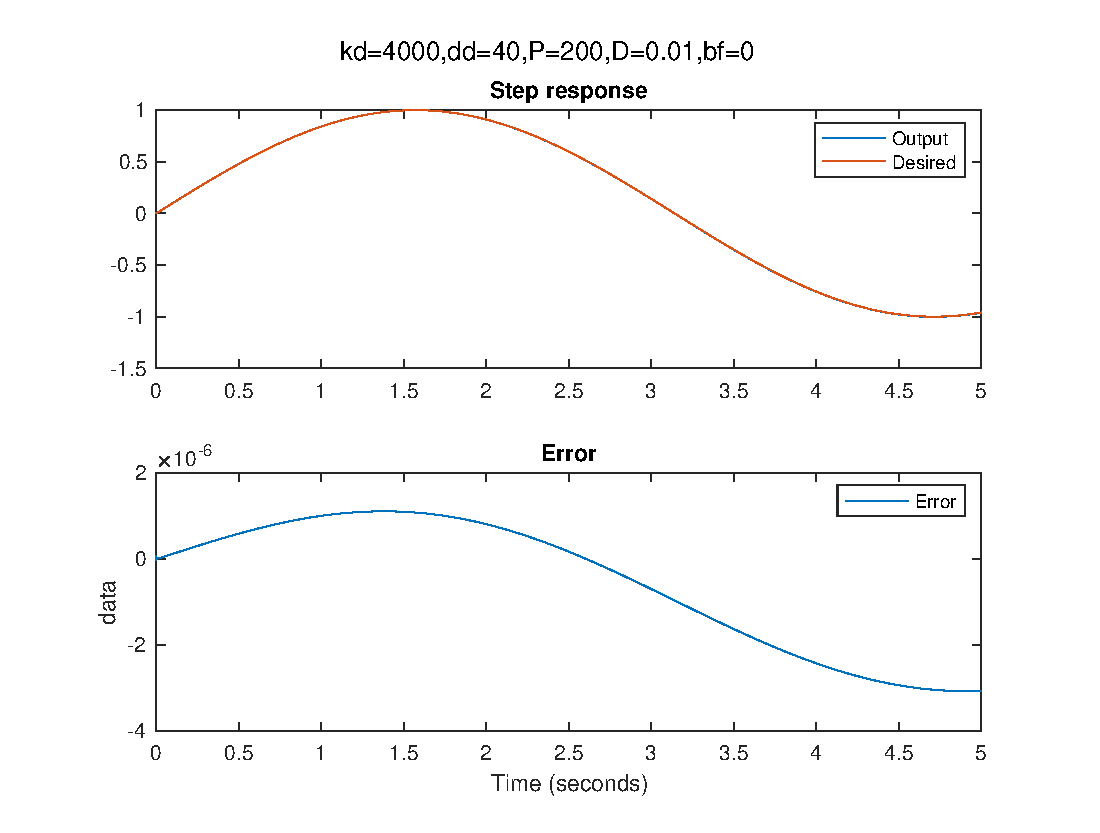
\includegraphics[width=8cm,height=8cm]{1.eps}}
    \end{subfigure}
    \hfill
        \begin{subfigure}[t]{0.4\textwidth}
        \raisebox{-\height}{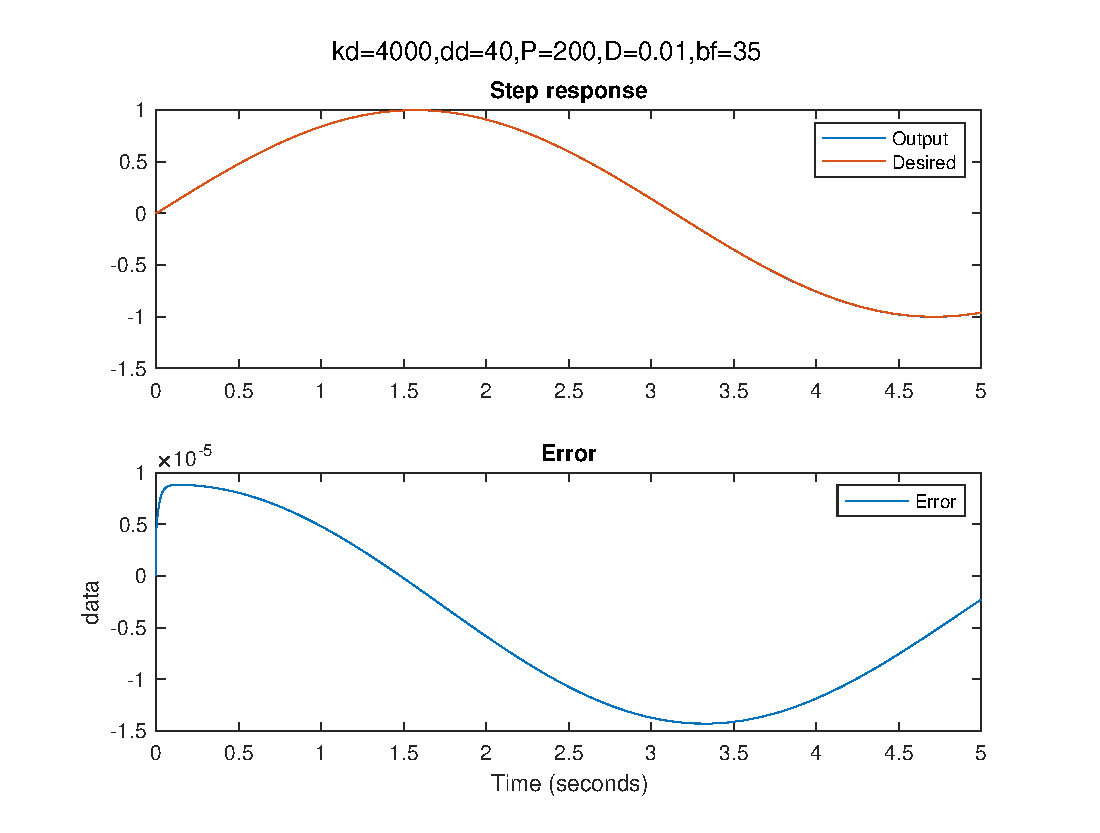
\includegraphics[width=8cm,height=8cm]{3.eps}}
    \end{subfigure}
    %%%%%%%%%%%%%%%%%%%%%%%%%%%%%%%%%%%%second row
    \begin{subfigure}[t]{0.4\textwidth}
        \raisebox{-\height}{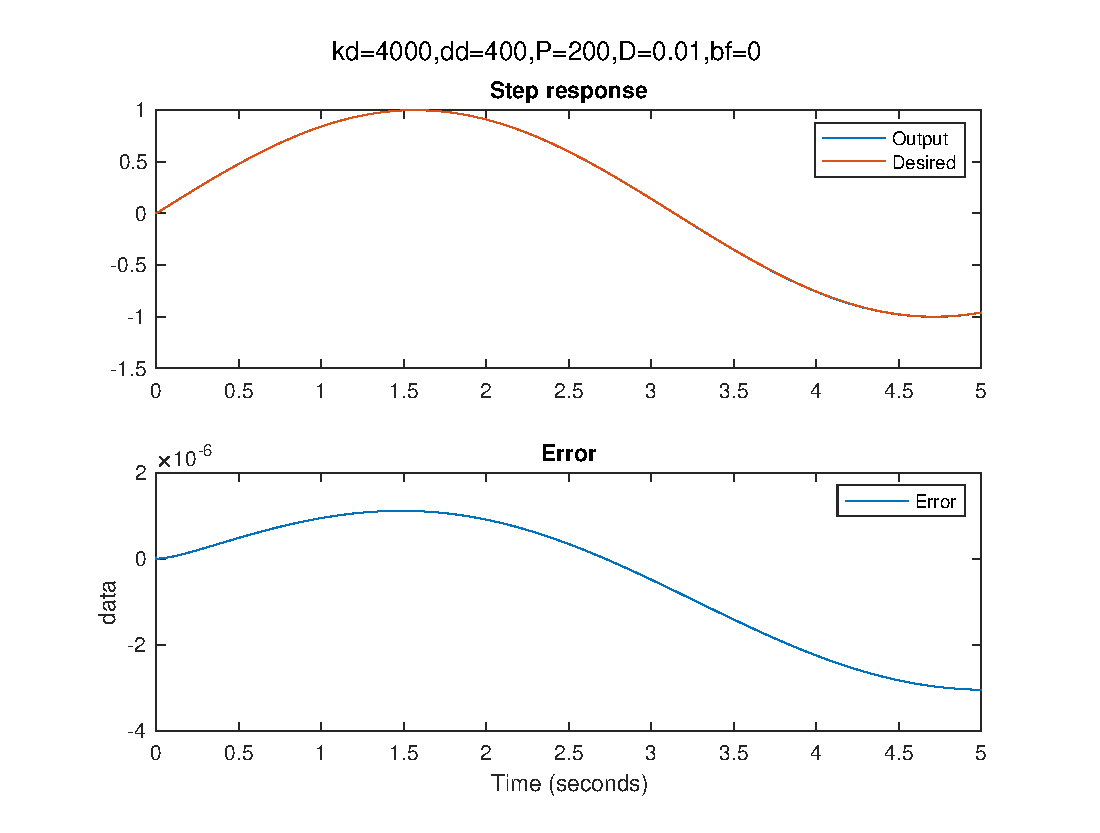
\includegraphics[width=8cm,height=8cm]{4.eps}}
    \end{subfigure}
    \hfill
        \begin{subfigure}[t]{0.4\textwidth}
        \raisebox{-\height}{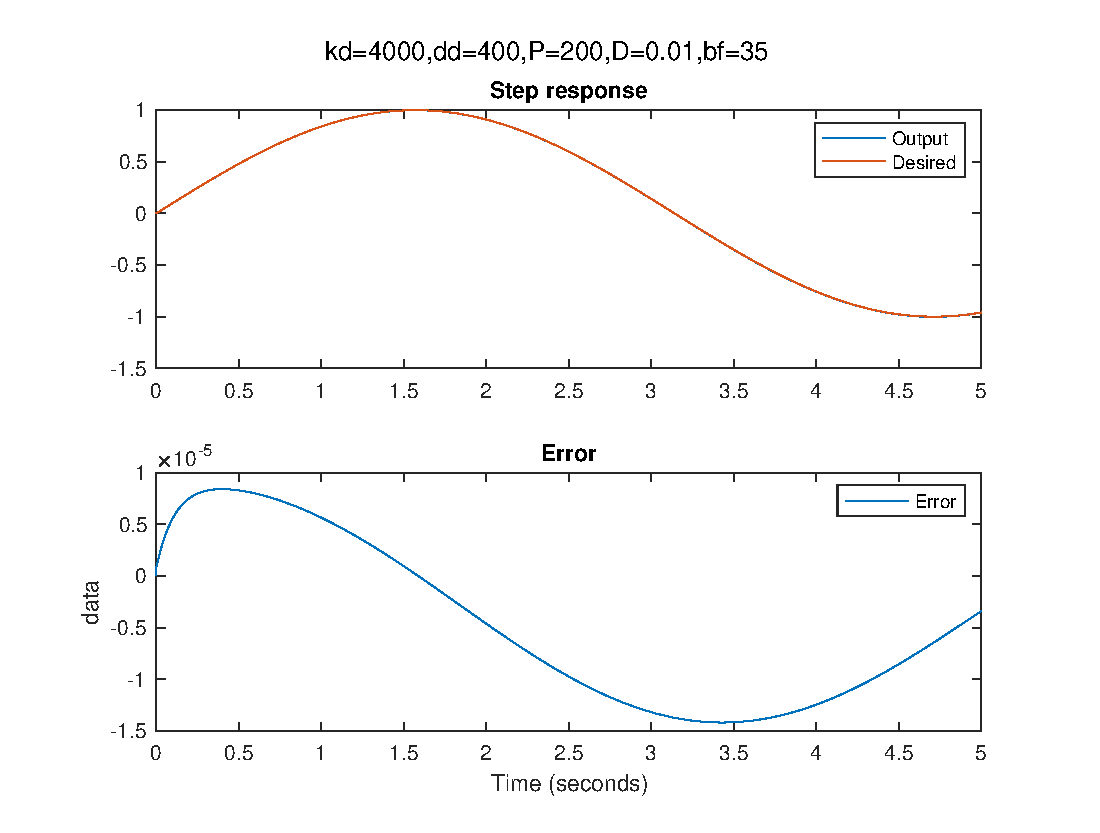
\includegraphics[width=8cm,height=8cm]{6.eps}}
        
    \end{subfigure}
        \begin{subfigure}[t]{0.4\textwidth}
        \raisebox{-\height}{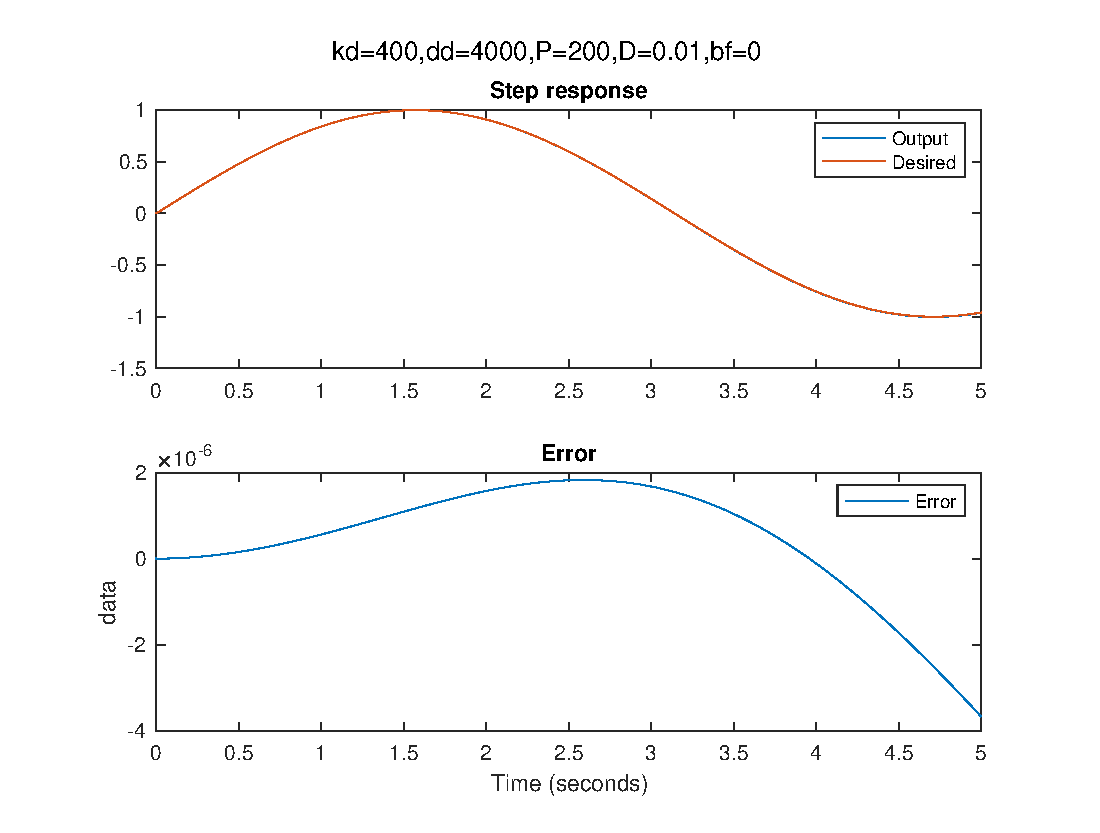
\includegraphics[width=8cm,height=8cm]{7.eps}}
    \end{subfigure}
    \hfill
        \begin{subfigure}[t]{0.4\textwidth}
        \raisebox{-\height}{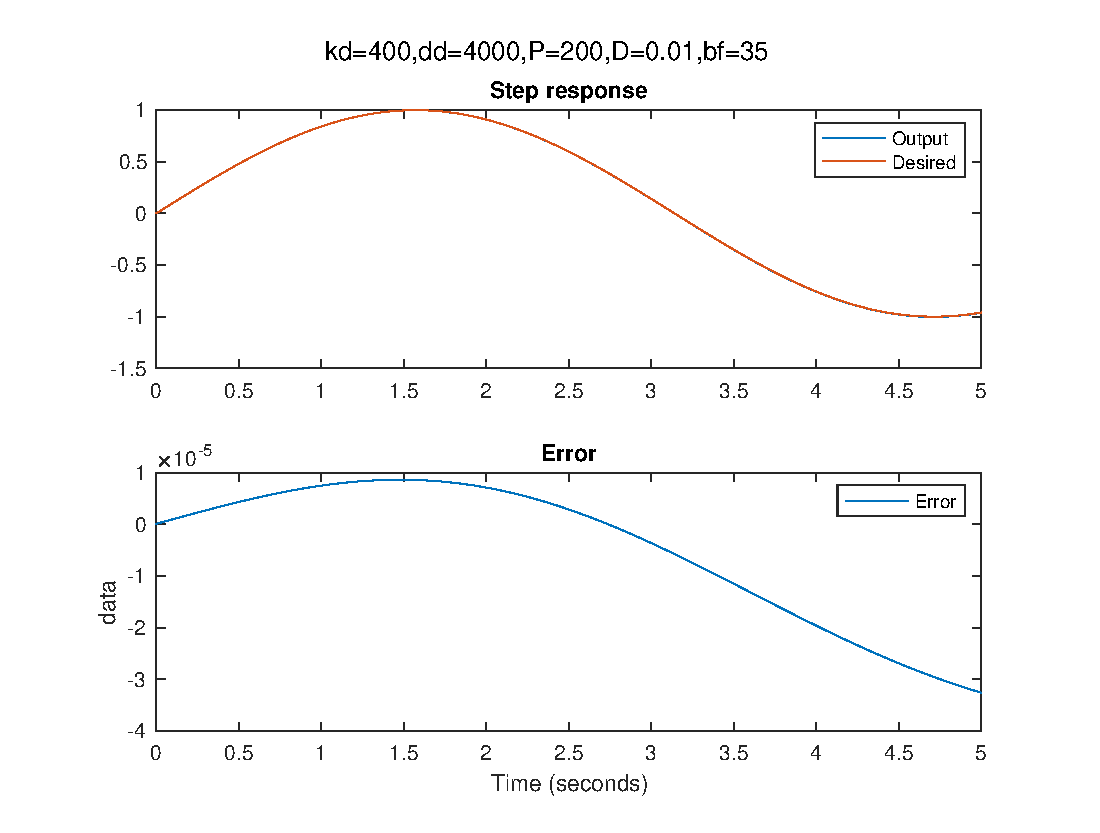
\includegraphics[width=8cm,height=8cm]{9.eps}}
    \end{subfigure}
    \caption{Performance of BIC for SEA and SDEA}
    \label{perf}
\end{figure}



\section{Conclusion}\\
Ensuring passivity of the control architecture is a necessary condition to ensure a stable interaction with any passive environment. In the exoskeleton systems, the environment is the human, which is assumed as a passive system\cite{hogan}. In VSIC architecture, it is not possible to passively render any desired impedance. A SEA with VSIC architecture cannot passively render a Voigt model\cite{tagliamonte}, which causes environment uncertainties\cite{calanca}.\\

Three different actuator is investigated through the research.The only difference between \textsc{HandsOn-SDEA} and \textsc{HandsOn-SEA} is a mechanical damper added parallel to the series elasticity in the mechanism. $b_f$ will have the value of damping in \textsc{HandsOn-SDEA}.However, $b_f$ is neglected in \textsc{HandsOn-SEA}, because there is no mechanical damper.\textsc{HandsOn-SDA} will sense the environment force by damping $b_f$.\\

For BIC, passivity constraints are derived for three different actuators.For SDA and SEA, since the force derivative gain D is usually small to avoid noise amplification, the proportional gain of force control is limited by derived conditions. The bandwith limit of the BIC controller depends on the actuator bandwith. Motor's mechanical resonance is an example for actuation bandwith limitation. Desired impedance is not limited for for $d_d$, but desired stiffness is limited by sensor's stiffness.\\

SDEA analysis provides constraints in selection of controller gains. Force control gains and desired impedance are limited by actuator's mass and sensor's stiffness and damping. There is an upper bound for sensing damping in terms of actuator's mass and damping. There is a relationship between sensor stiffness and desired stiffness. Lower inertia allows the system to be able render higher stiffness than its own.\\



\section{Future Work}\\
SDEA and SDA are type of actuators that emerge to be investigated according to passivity. Another controllers can be implemented on those actuators, such as motion controlled admittance display,generic controller. Analysis and comparision of passivity constraint of the SEA/SDEA/SDA might be a good research topic to be covered for different controller architectures and desired impedances.

\begin{figure}
     \centering
    \begin{subfigure}[t]{0.4\textwidth}
        \raisebox{-\height}{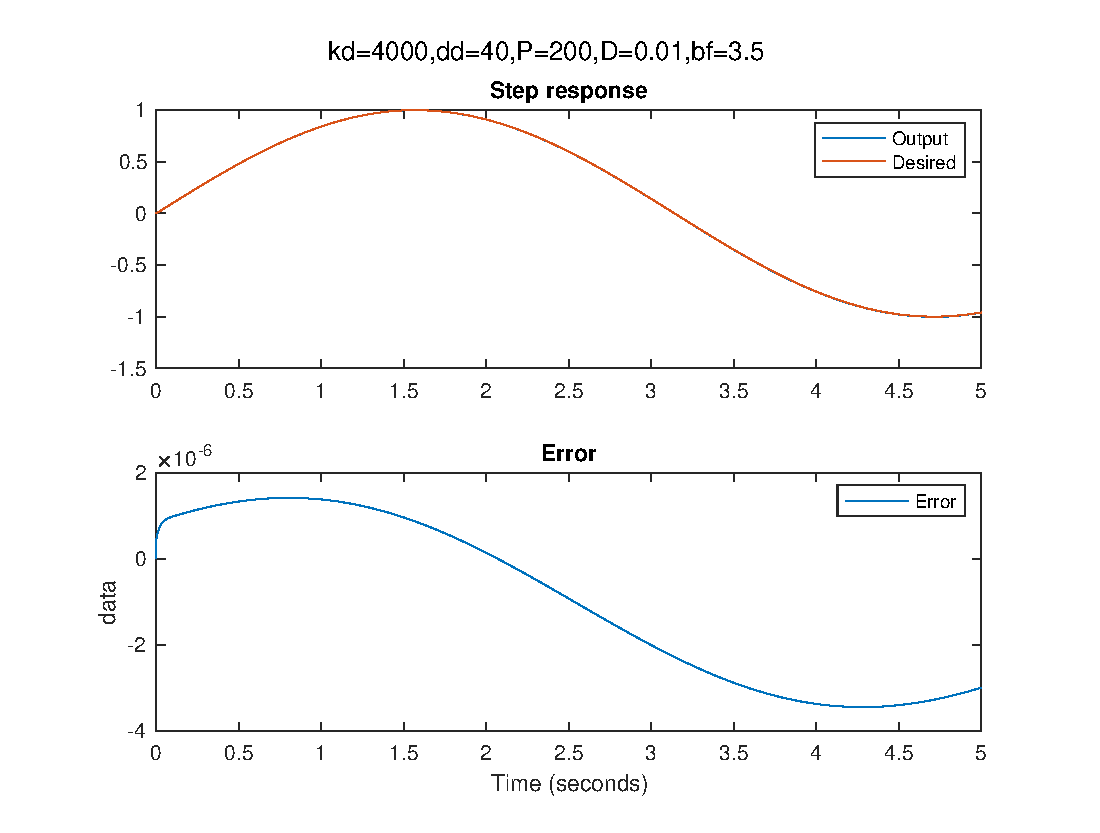
\includegraphics[width=8cm,height=8cm]{a.eps}}
    \end{subfigure}
    \hfill
        \begin{subfigure}[t]{0.4\textwidth}
        \raisebox{-\height}{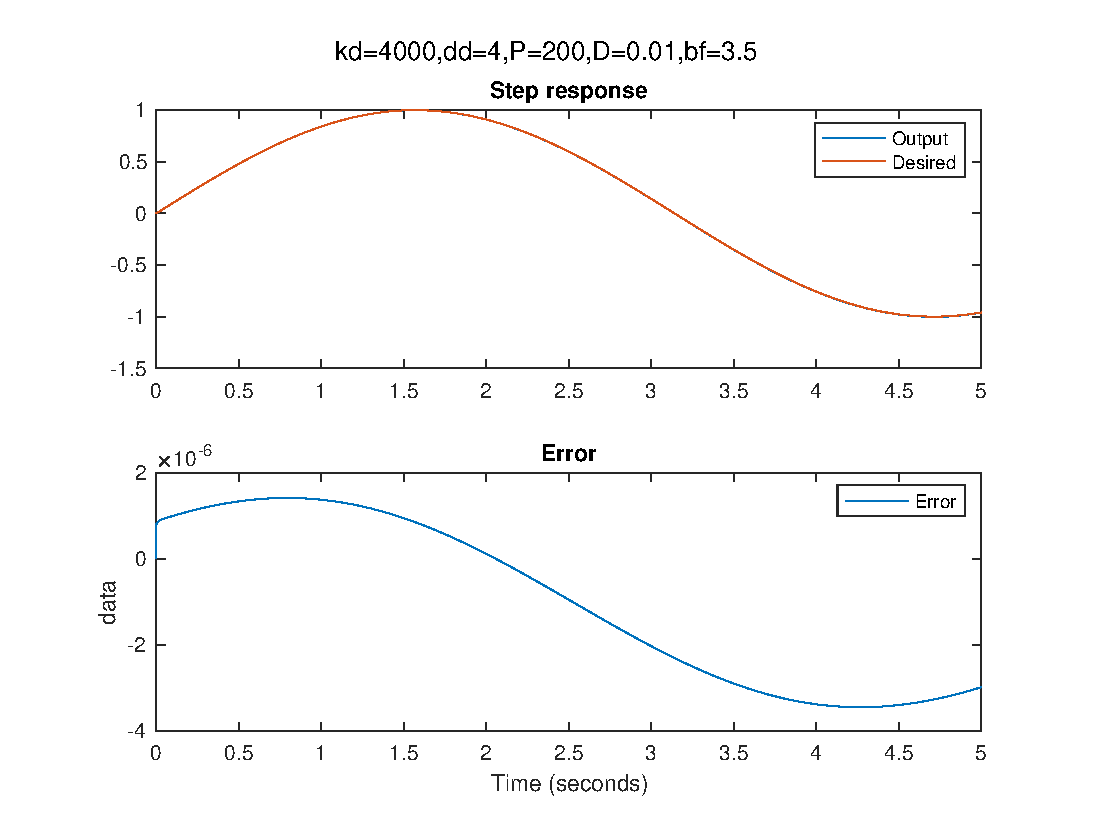
\includegraphics[width=8cm,height=8cm]{b.eps}}
    \end{subfigure}
    %%%%%%%%%%%%%%%%%%%%%%%%%%%%%%%%%%%%second row
    \begin{subfigure}[t]{0.4\textwidth}
        \raisebox{-\height}{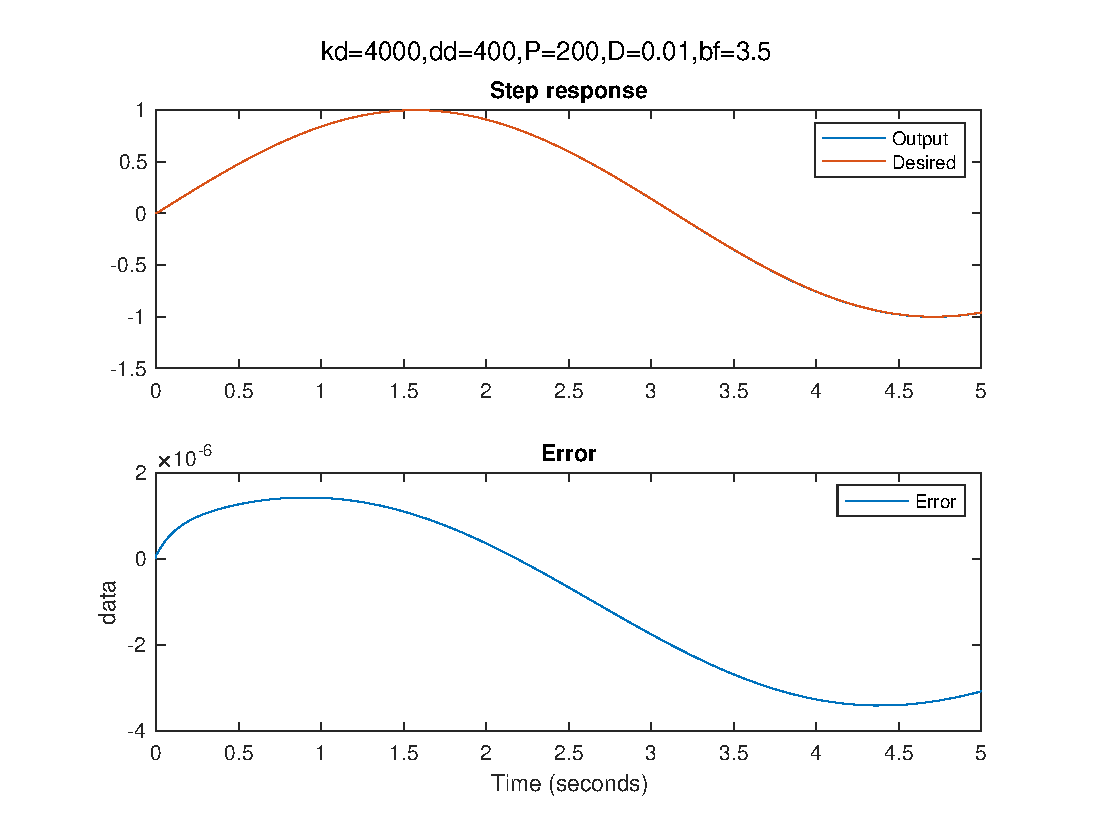
\includegraphics[width=8cm,height=8cm]{c.eps}}
    \end{subfigure}
    \hfill
        \begin{subfigure}[t]{0.4\textwidth}
        \raisebox{-\height}{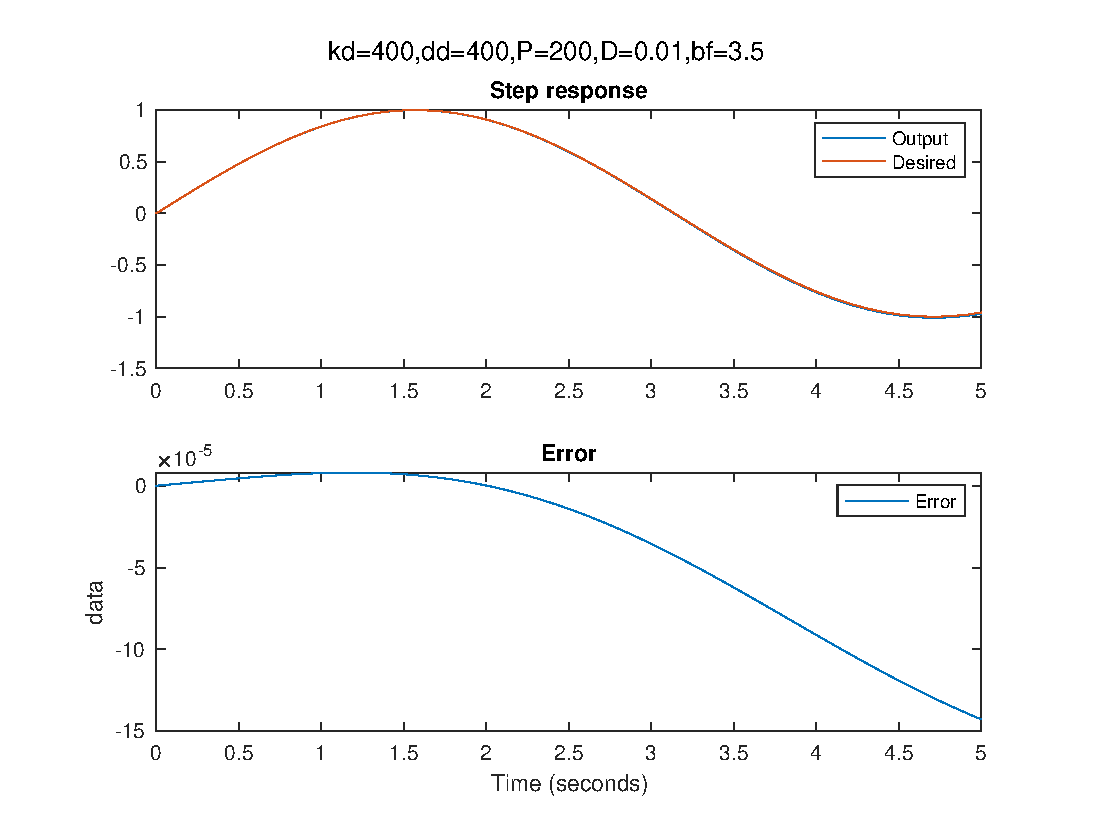
\includegraphics[width=8cm,height=8cm]{d.eps}}
        
    \end{subfigure}
        \begin{subfigure}[t]{0.4\textwidth}
        \raisebox{-\height}{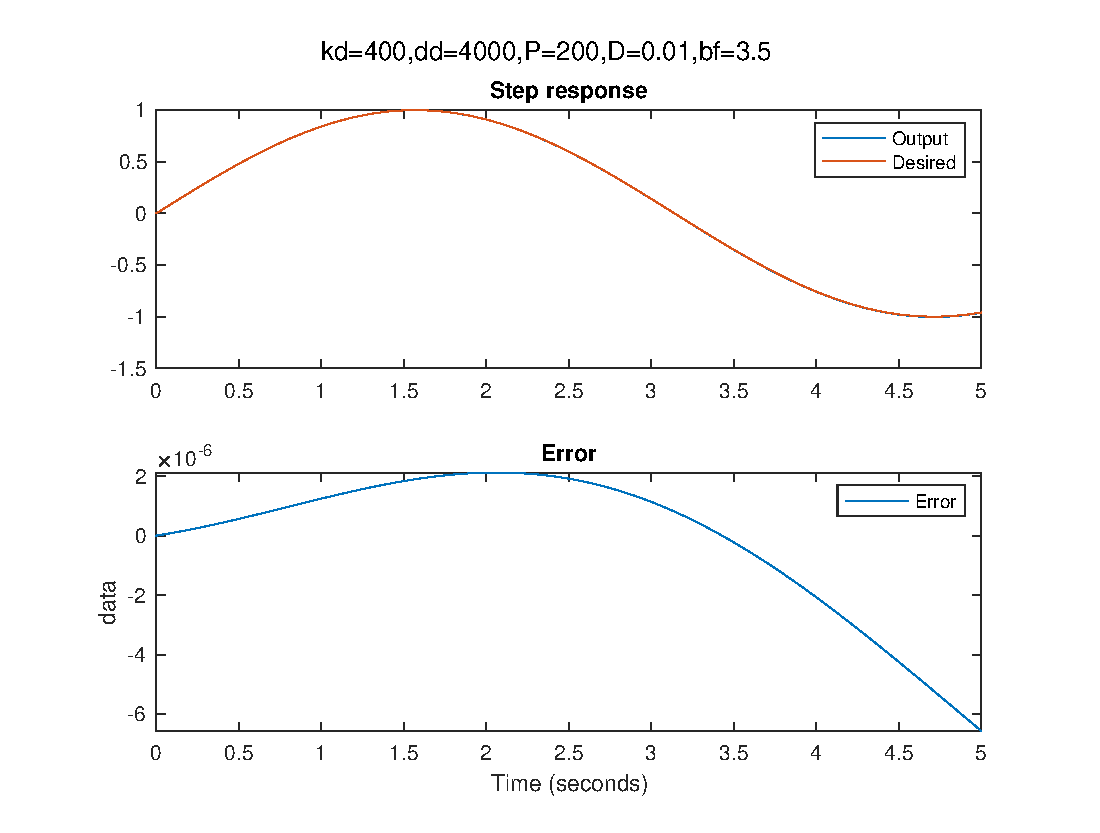
\includegraphics[width=8cm,height=8cm]{e.eps}}
    \end{subfigure}
    \hfill
        \begin{subfigure}[t]{0.4\textwidth}
        \raisebox{-\height}{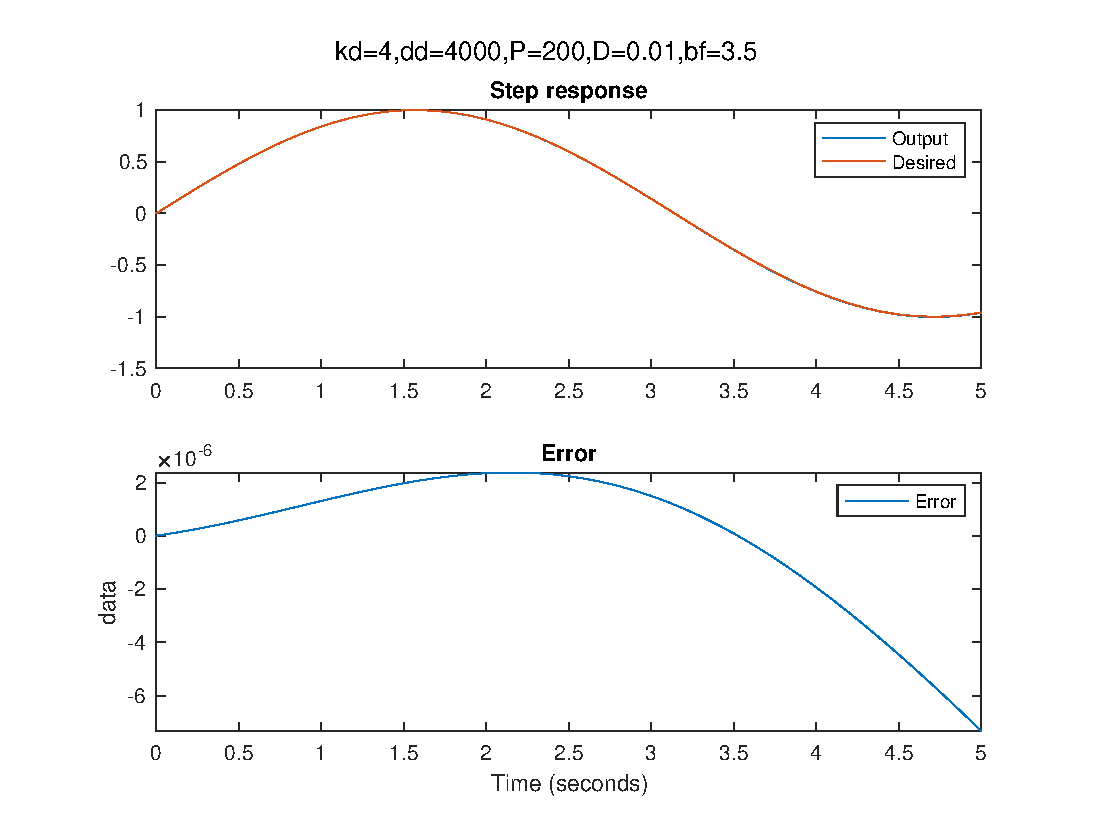
\includegraphics[width=8cm,height=8cm]{f.eps}}
    \end{subfigure}
    \caption{Performance of BIC for SDEA}
    \label{perf2}
\end{figure}
\newpage
\printbibliography



\end{document}